\documentclass[a4paper,11pt]{article}
\usepackage[a4paper, margin=8em]{geometry}

% usa i pacchetti per la scrittura in italiano
\usepackage[french,italian]{babel}
\usepackage[T1]{fontenc}
\usepackage[utf8]{inputenc}
\frenchspacing 

% usa i pacchetti per la formattazione matematica
\usepackage{amsmath, amssymb, amsthm, amsfonts}

% usa altri pacchetti
\usepackage{gensymb}
\usepackage{hyperref}
\usepackage{standalone}

% imposta il titolo
\title{Modello di Drude-Lorentz}
\author{Luca Seggiani}
\date{2026}

% imposta lo stile
% usa helvetica
\usepackage[scaled]{helvet}
% usa palatino
\usepackage{palatino}
% usa un font monospazio guardabile
\usepackage{lmodern}

\renewcommand{\rmdefault}{ppl}
\renewcommand{\sfdefault}{phv}
\renewcommand{\ttdefault}{lmtt}

% disponi il titolo
\makeatletter
\renewcommand{\maketitle} {
	\begin{center} 
		\begin{minipage}[t]{.8\textwidth}
			\textsf{\LARGE\bfseries \@title} 
		\end{minipage}%
		\begin{minipage}[t]{.2\textwidth}
			\raggedleft \vspace{-1.65em}
			\textsf{\small \@author} \vfill
			\textsf{\small \@date}
		\end{minipage}
		\par
	\end{center}

	\thispagestyle{empty}
	\pagestyle{fancy}
}
\makeatother

% disponi teoremi
\usepackage{tcolorbox}
\newtcolorbox[auto counter, number within=section]{theorem}[2][]{%
	colback=blue!10, 
	colframe=blue!40!black, 
	sharp corners=northwest,
	fonttitle=\sffamily\bfseries, 
	title=~\thetcbcounter: #2, 
	#1
}

% disponi definizioni
\newtcolorbox[auto counter, number within=section]{definition}[2][]{%
	colback=red!10,
	colframe=red!40!black,
	sharp corners=northwest,
	fonttitle=\sffamily\bfseries,
	title=~\thetcbcounter: #2,
	#1
}

% U.D.M
\newcommand{\amp}{\ensuremath{\mathrm{A}}}
\newcommand{\volt}{\ensuremath{\mathrm{V}}}
\newcommand{\meter}{\ensuremath{\mathrm{m}}}
\newcommand{\second}{\ensuremath{\mathrm{s}}}
\newcommand{\farad}{\ensuremath{\mathrm{F}}}
\newcommand{\henry}{\ensuremath{\mathrm{H}}}
\newcommand{\siemens}{\ensuremath{\mathrm{S}}}

% circuiti
\usepackage{circuitikz}
\usetikzlibrary{babel}

% disegni
\usepackage{pgfplots}
\pgfplotsset{width=10cm,compat=1.9}

% disponi codice
\usepackage{listings}
\usepackage[table]{xcolor}

\definecolor{codegreen}{rgb}{0,0.6,0}
\definecolor{codegray}{rgb}{0.5,0.5,0.5}
\definecolor{codepurple}{rgb}{0.58,0,0.82}
\definecolor{backcolour}{rgb}{0.95,0.95,0.92}

\lstdefinestyle{codestyle}{
		backgroundcolor=\color{black!5}, 
		commentstyle=\color{codegreen},
		keywordstyle=\bfseries\color{magenta},
		numberstyle=\sffamily\tiny\color{black!60},
		stringstyle=\color{green!50!black},
		basicstyle=\ttfamily\footnotesize,
		breakatwhitespace=false,         
		breaklines=true,                 
		captionpos=b,                    
		keepspaces=true,                 
		numbers=left,                    
		numbersep=5pt,                  
		showspaces=false,                
		showstringspaces=false,
		showtabs=false,                  
		tabsize=2
}

\lstdefinestyle{shellstyle}{
		backgroundcolor=\color{black!5}, 
		basicstyle=\ttfamily\footnotesize\color{black}, 
		commentstyle=\color{black}, 
		keywordstyle=\color{black},
		numberstyle=\color{black!5},
		stringstyle=\color{black}, 
		showspaces=false,
		showstringspaces=false, 
		showtabs=false, 
		tabsize=2, 
		numbers=none, 
		breaklines=true
}

\lstdefinelanguage{javascript}{
	keywords={typeof, new, true, false, catch, function, return, null, catch, switch, var, if, in, while, do, else, case, break},
	keywordstyle=\color{blue}\bfseries,
	ndkeywords={class, export, boolean, throw, implements, import, this},
	ndkeywordstyle=\color{darkgray}\bfseries,
	identifierstyle=\color{black},
	sensitive=false,
	comment=[l]{//},
	morecomment=[s]{/*}{*/},
	commentstyle=\color{purple}\ttfamily,
	stringstyle=\color{red}\ttfamily,
	morestring=[b]',
	morestring=[b]"
}

% disponi sezioni
\usepackage{titlesec}

\titleformat{\section}
	{\sffamily\Large\bfseries} 
	{\thesection}{1em}{} 
\titleformat{\subsection}
	{\sffamily\large\bfseries}   
	{\thesubsection}{1em}{} 
\titleformat{\subsubsection}
	{\sffamily\normalsize\bfseries} 
	{\thesubsubsection}{1em}{}

% disponi alberi
\usepackage{forest}

\forestset{
	rectstyle/.style={
		for tree={rectangle,draw,font=\large\sffamily}
	},
	roundstyle/.style={
		for tree={circle,draw,font=\large}
	}
}

% disponi algoritmi
\usepackage{algorithm}
\usepackage{algorithmic}
\makeatletter
\renewcommand{\ALG@name}{Algoritmo}
\makeatother

% disponi numeri di pagina
\usepackage{fancyhdr}
\fancyhf{} 
\fancyfoot[L]{\sffamily{\thepage}}

\makeatletter
\fancyhead[L]{\raisebox{1ex}[0pt][0pt]{\sffamily{\@title \ \@date}}} 
\fancyhead[R]{\raisebox{1ex}[0pt][0pt]{\sffamily{\@author}}}
\makeatother

\begin{document}

\pagestyle{fancy}
\thispagestyle{empty}
\renewcommand{\thispagestyle}[1]{}

\maketitle

Nei corsi di fisica ed elettronica la trattazione del fenomeno di conduzione all'interno di un materiale metallico (o facendo le dovute considerazioni, in un semiconduttore che fornisce elettroni liberi) viene fatta attraverso il modello di \textbf{Drude-Lorentz}. Questo è un modello che studia a livello microscopico il comportamento dei portatori di carica (elettroni nel caso di metalli, elettroni e lacune nel caso di semiconduttori) assumendoli come gas ideali governati dalle leggi della meccanica. Presentiamo qui una breve trattazione del modello e 2 simulazioni numeriche che ne verificano la validità.

\section{Trattazione analitica}

Alla base del modello di Drude-Lorentz sta la definizione di una certa \textbf{velocità di deriva} $\vec{v}_d$. Questa viene definita come la velocità media di un dato elettrone all'interno del reticolo reticolo elettronico considerato, sottoposto ad un campo elettrico $\vec{E}$. 

Assumiamo quindi gli elettroni come particelle di carica $-e$ e massa $m$. In tal caso la forza a cui saranno sottoposti sotto il campo $\vec{E}$ sarà data dalla \textbf{legge di Coulomb}, da cui è immediata anche l'accelerazione:
$$
\vec{F} = -e \vec{E}, \quad \vec{a} = -\frac{e \vec{E}}{m}
$$

Prendiamo il moto del singolo elettrone come stazionario al tempo $t_0 = 0$. Da qui in poi, questo si muoverà di moto uniformememente accelerato nella direzione del campo, a cui si somma una componente casuale di origine termica. Diciamo ad ogni collisione $i$, la velocità a $\vec{v}_{i}$ accumulata fino a tal punto sarà data da:
$$
\vec{v}_i = \vec{v}_{i - 1} - \frac{e \vec{E}}{m} t_i = \vec{v}_{i - 1} + a t_i
$$
dove $\vec{v}_{i - 1}$ sarà la velocità accumulata per eccitazione termica nel corso del moto dell'elettrone, e il termine $\frac{e \vec{E}}{m} t_i$ rappresenterà la velocità accumulata per l'accelerazione del campo elettrico in un \textbf{tempo di cammino} (o \textit{cammino libero}) $t_i$. Immaginiamo che avvenuta la collisione, la velocità istantanea $\vec{v}$ dell'elettrone si pone a 0, e il processo ricomincia da capo.

Il processo descritto è \textit{stocastico} in quanto il tempo di cammino $t_i$ non è predeterminato, ma casuale e governato dalle caratteristiche del modello del \textit{mare di elettroni} in un conduttore come gas. In particolare, si ha che la distribuzione di probabilità dei tempi di cammino è di tipo esponenziale, con funzione densità di probabilità:
$$
P(t) = \frac{1}{\tau} e^{-\frac{t}{\tau}}
$$
dove $\tau$ è il \textbf{tempo di cammino medio} (o \textit{cammino libero medio}) all'interno del materiale considerato.

Il risultato che si trova (e verificheremo numericamente nelle prossime sezioni) è che le velocità $\vec{v}_{i - 1}$, casuali e determinate dall'eccitazione termica, hanno contributo complessivo nullo, mentre le velocità $\frac{e \vec{E}}{m} t_i$ si accumulano, dando una velocità di deriva:
$$
\vec{v}_d = < \vec{v}_i > = -\frac{e \vec{E}}{m} \tau = \vec{a} \tau
$$

La valenza del modello di Drude-Lorentz si ha dal fatto che, posta la \textbf{mobilità elettronica} $\mu_n$ come:
$$
\mu_n = \frac{e \tau}{m}, \quad \vec{v}_d = -\mu_n \vec{E}
$$
si ricava un'espressione microscopica per la \textbf{legge di Ohm}, che permette di riportare il comportamento macroscopico dei conduttori alle proprietà dei singoli elettroni nel materiale:
$$
\vec{J} = -n e \vec{v}_d = n e \mu_n \vec{E}
$$
dove $\vec{J}$ è la densità di corrente e $n$ è la densità elettronica. Questo si riporta ad una definizione di corrente dalla definizione:
$$
\vec{I} = \frac{\vec{J}}{S} = \frac{n e \mu_n \vec{E}}{S}
$$
da cui si ha fra l'altro una definizione in termini microscopici della \textit{conduttanza}, data dalle caratteristiche dei materiali cosiddetti \textit{Ohmici}:
$$
\vec{J} = \sigma \vec{E}, \quad \sigma = n e \mu_n
$$

Potremmo chiederci come mai si prende come valore della velocità di deriva:
$$
\vec{v}_d = \vec{a} \tau \neq \frac{1}{2} \vec{a} \tau
$$
e non la sua metà. Questo risulterebbe infatti valido dal fatto che l'andamento della velocità dell'elettrone, dato il suo comportamento dove si ferma e riparte, è un onda a dente di sega, di cui l'integrale è chiaramente la metà del modulo. 

Cercheremo quindi di ricavare questo risultato in maniera numerica. Da qui in poi trascureremo il segno negativo alla carica dell'elettrone $-e$, in quanto siamo interessati ai moduli delle grandezze vettoriali considerate. Inoltre, trascureremo i termini di velocità $\vec{v}_{i - 1}$ di eccitazione termica in quanto, come abbiamo detto, questi possono essere trascurati preso un intervallo temporale abbastanza grande (si annullano fra di loro nel tempo). Questo ci permette di riportare tutto il modello da uno spazio vettoriale tridimensionale ad uno monodimensionale, dove l'unica traslazione effettivamente importante è quella nella direzione del campo $\vec{E}$.

\section{Modello a singolo elettrone}
Vediamo quindi un primo modello. Questo si basa sul prendere un singolo elettrone e simularlo nel tempo. Si simula quindi l'accelerazione nel tempo secondo il termine di accelerazione:
$$
a = \frac{q E}{m}
$$
e le collisioni (che annullano la velocità dell'elettrone), che si verificano dopo un tempo di cammino $t_i$. Questo viene calcolato a partire dalla distribuzione di probabilità esponenziale con funzione densità di probabilità:
$$
P(t) = \frac{1}{\tau} e^{-\frac{t}{\tau}}
$$

Vediamo quindi una simulazione che usa uno schema di integrazione di Eulero semi-implicito per calcolare velocità e spostamento complessivo dell'elettrone nel tempo. Questa andrà a riempire due vettori, $\mathbf{v}$ e $\mathbf{s}$, contenenti rispettivamente le velocità e gli spostamenti dell'elettrone per ogni istante $i$. Gli istanti $i$ verranno distanziati da un $\Delta$ determinato come:
$$
\Delta = \frac{\text{max}_\text{time}}{\text{steps}}
$$
cioè un tempo massimo di simulazione sul numero di passaggi che vogliamo effetuare. 
Le equazioni del moto che vorremo implementare saranno:
$$
\begin{cases}
	\mathbf{v}_i = 
	\begin{cases}
		0, & \text{se c'è collisione} \\
		\mathbf{v}_{i - 1} + a \Delta, & \text{altrimenti}
	\end{cases} 
	\\
	\mathbf{s}_i = \mathbf{s}_{i - 1} + \mathbf{v}_i \Delta
\end{cases}
$$
Lo schema risulta quindi non puramente semi-implicito, in quanto c'è una discontinuità data dalle collisioni. Uno script Python che implementerà la simulazione potrà essere:
\begin{lstlisting}[language=python, style=codestyle]
import numpy as np
import matplotlib.pyplot as plt

# probability constants
tau = 2.5 * 10 ** -14

# gets random flight time
def get_coll():
    return np.random.exponential(scale=tau)

# time constants
max_time = 10 ** -12
steps = 10000
delta = max_time / (steps - 1)

# physical constants
q = 1.6 * 10 ** -19
E = 1
m = 9.3 * 10 ** -31
a = (q * E) / m

# state variables
s = np.zeros(steps)
v = np.zeros(steps)

# simulate
next_coll = get_coll()
for i in range(1, steps):
    time = i * delta

    # velocity
    v[i] = v[i - 1] + a * delta
    while time > next_coll:
        # collide
        v[i] = 0
        next_coll += get_coll() 

    # position
    s[i] = s[i - 1] + v[i] * delta
\end{lstlisting}

L'esecuzione di questo script porterà alla popolazione di due vettori \lstinline|s| e \lstinline|v| corrispondenti ai vettori $\mathbf{s}$ e $\mathbf{v}$ degli spostamenti e delle velocità rispettivamente. 

\newpage

Graficando la velocità e lo spostamento dell'elettrone si avranno i seguenti grafici:
\begin{figure}[H]
\centering
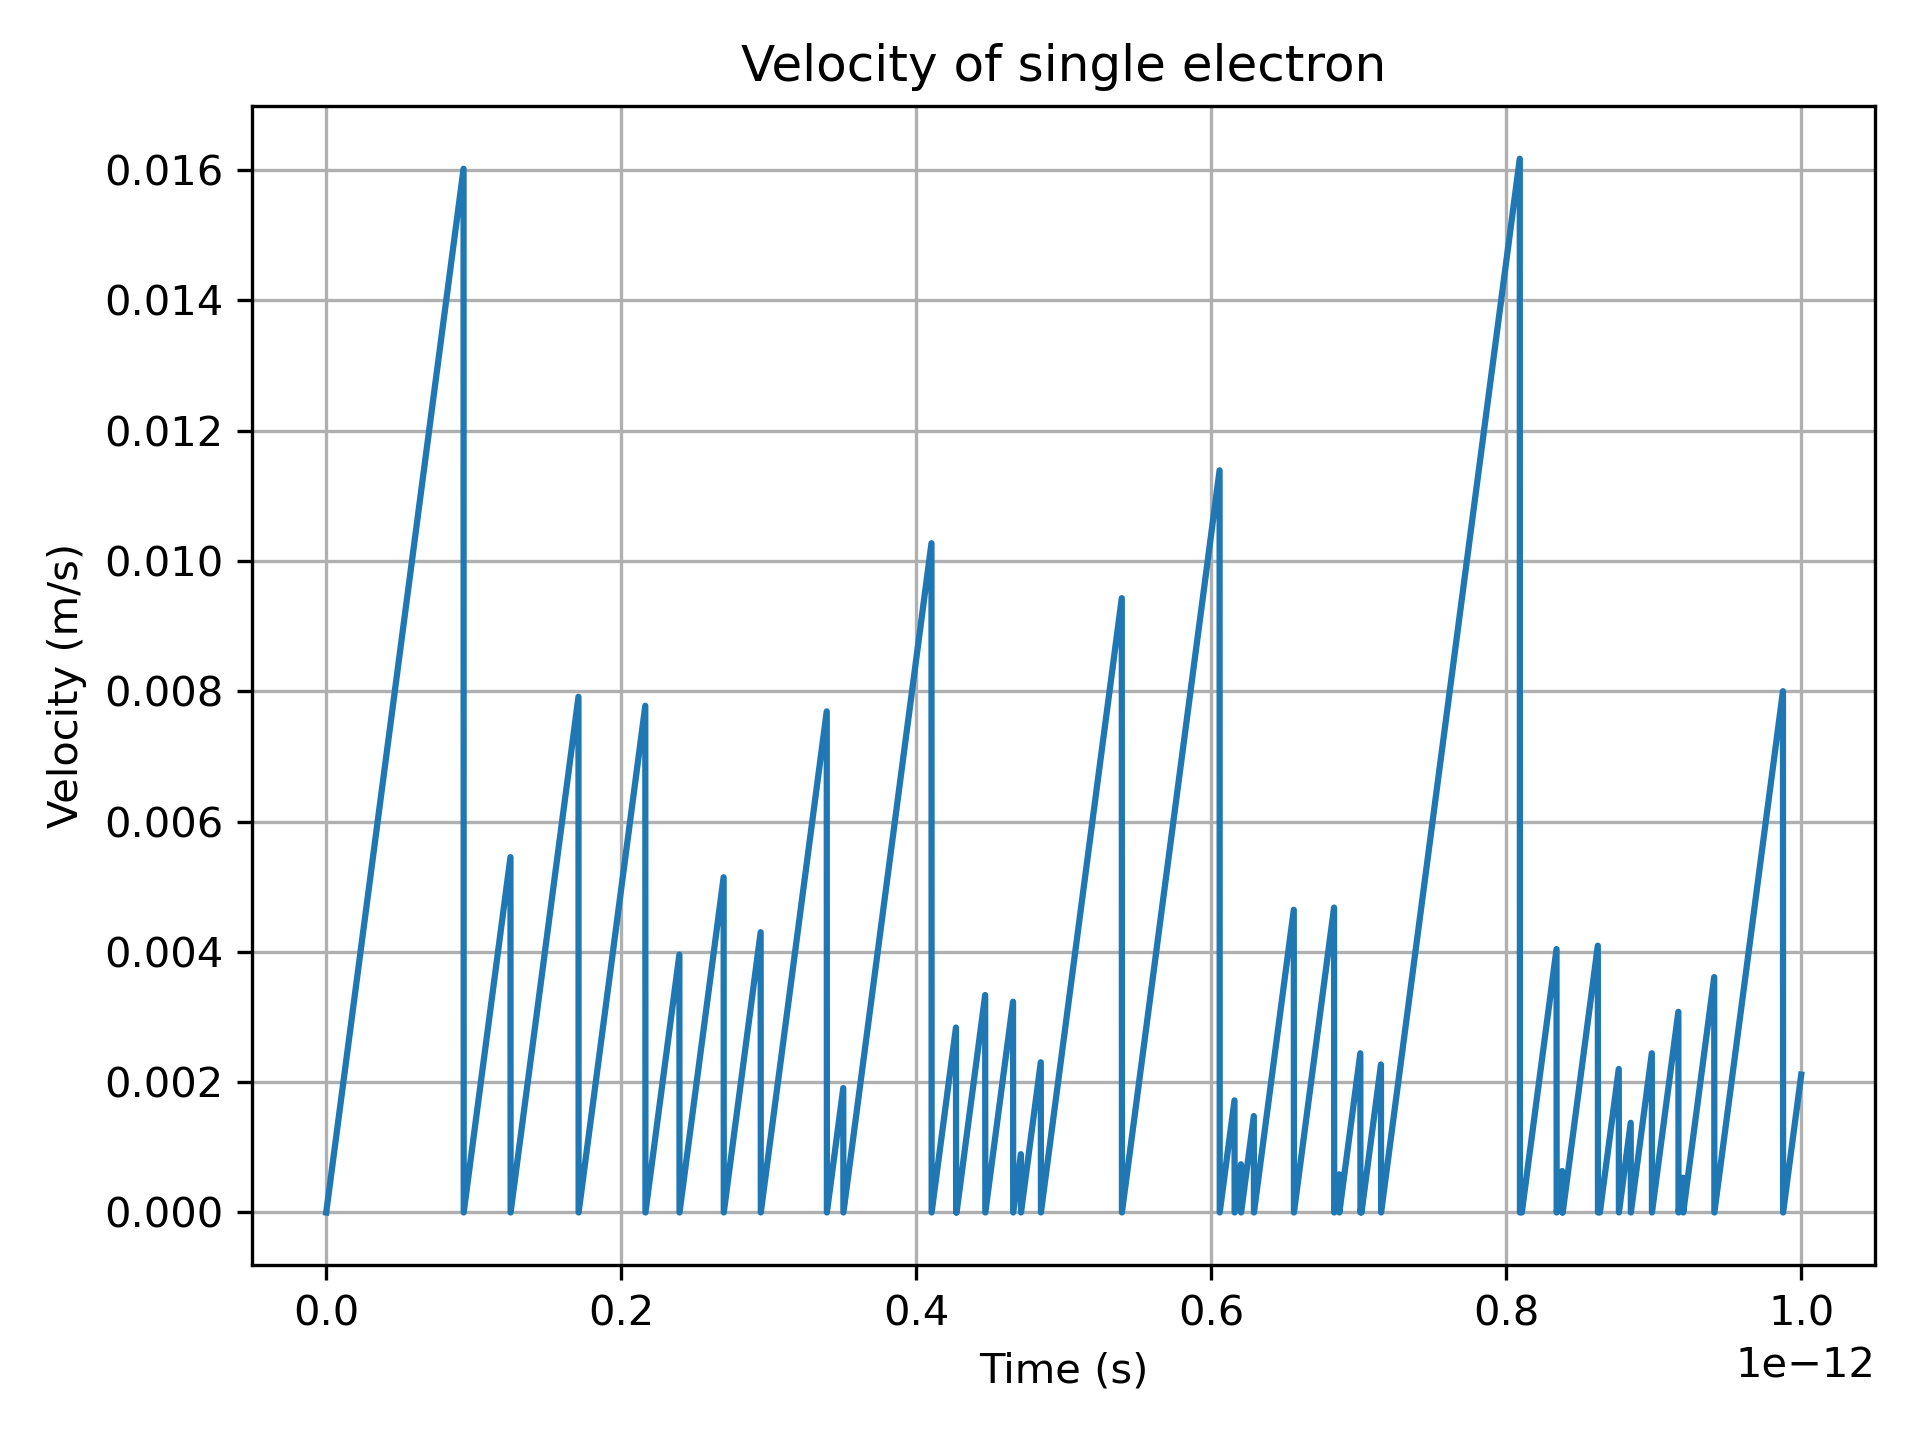
\includegraphics[width=0.48\textwidth]{figures/single_electron_velocity.png}
\hfill
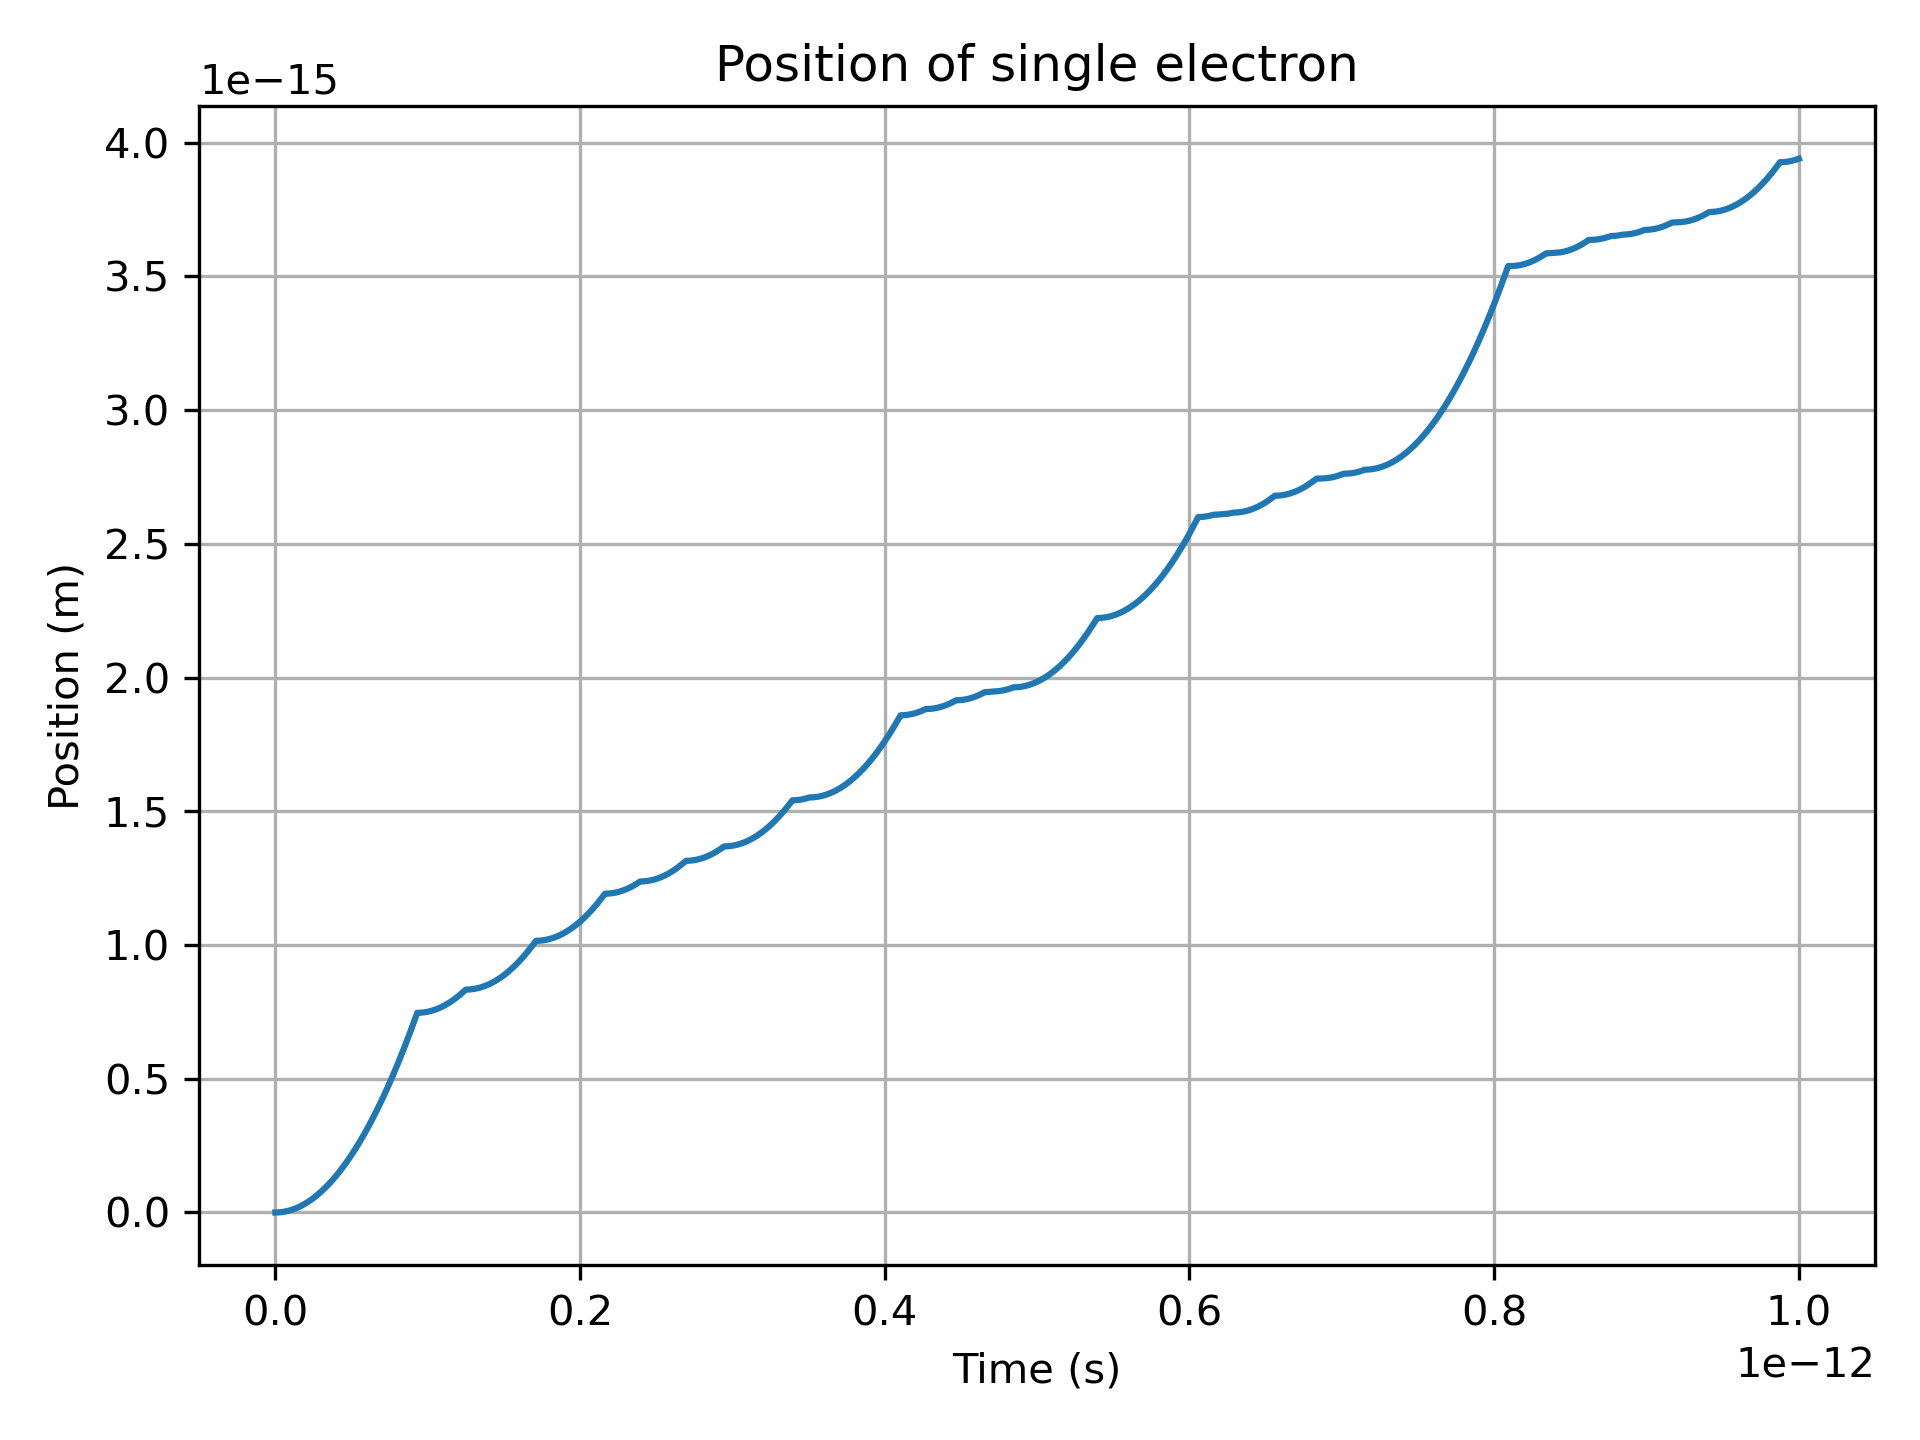
\includegraphics[width=0.48\textwidth]{figures/single_electron_position.png}
\end{figure}
da cui si nota l'andamento a "dente di sega" della velocità, e il corrispettivo comportamento dello spostamento, cioè l'elettrone tende a percorrere una certa distanza (con andamento quadratico dato da $\frac{1}{2} a t^2$), quindi a fermarsi (in corrispondenza di collisioni), e a ripartire.

Graficando la distribuzione delle velocità come istogramma si ha il seguente grafico:
\begin{figure}[H]
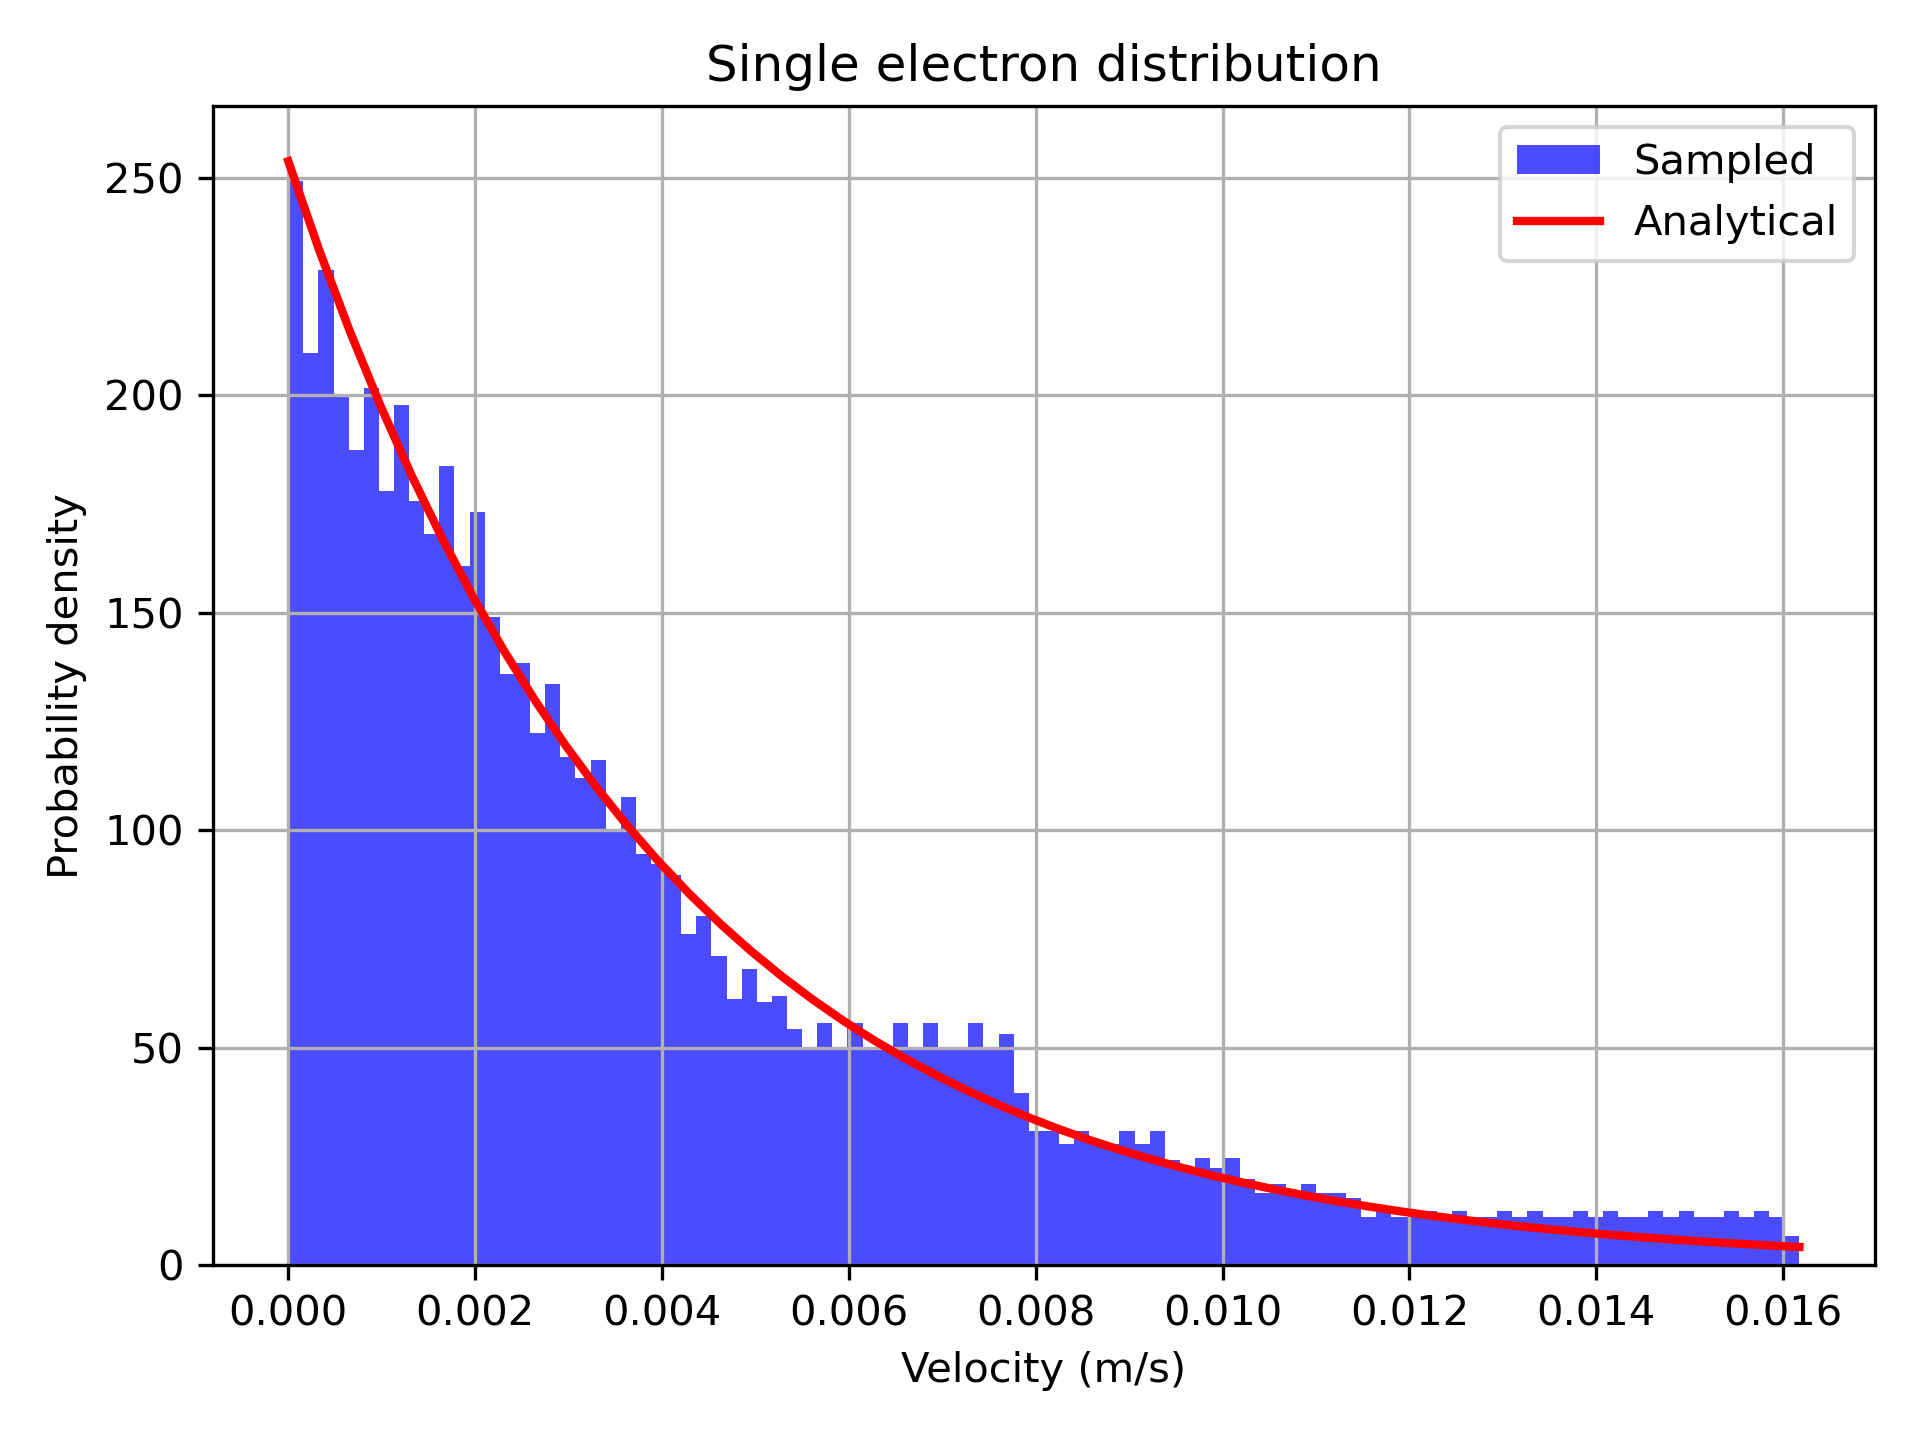
\includegraphics[width=0.96\textwidth]{figures/single_electron_distrib.png}
\end{figure}
Su questo grafico è stata messa a confronto la funzione densità di probabilita della distribuzione di probabilità esponenziale con media $v_d$, cioè corrispondente alla velocità di deriva teorizzata:
$$
P(v) = \frac{1}{v_d} e^{-\frac{v}{v_d}} , \quad v_d = \frac{q E}{m} \tau = \alpha t
$$
per cui abbiamo che il modello sviluppato è in accordo con il risultato teorico, e la velocità di deriva risulta uguale all'accelerazione $a$ per il tempo di cammino medio $\tau$.

\section{Modello a più elettroni}
Potremmo pensare di effettuare la simulazione seguendo una via diversa. Anziché simulare un singolo elettrone con tempo di cammino campionato casualmente dalla distribuzione di probabilità esponenziale, simuliamo più elettroni con tempo di cammino costante, campionato sempre da una certa distribuzione di probabilità $P'(t)$, tarata sulla probabilità di trovare un elettrone con dato tempo di cammino dalla sua ultima collisione fra tutti quelli nel \textit{mare di elettroni}. Prendiamo tale distribuzione di probabilità come proporzionale alla distribuzione $P(t)$ dei tempi di cammino, moltiplicata per il tempo di cammino stesso:
$$
P'(t) \propto t P(t) = \frac{t}{\tau} e^{-\frac{t}{\tau}}
$$
Questo è giustificato dal fatto che la probabilità di trovare un elettrone con dato tempo di cammino dipende dal tempo che quell'elettrone trascorre con tale tempo di cammino. Questo tempo sarà chiaramente il tempo di cammino stesso, per cui si scala per $t$. Abbiamo poi che la $P'(t)$ proposta, così com'è, non è normalizzata. Si dimostra analiticamente che l'integrale va a $\tau$:
$$
\int_0^\infty \frac{t}{\tau} e^{-\frac{t}{\tau}} \, dt = \tau
$$
per cui si normalizza dividendo per $\tau$, ottenendo la formula definitiva per la $P'(t)$:
$$
P'(t) = \frac{t}{\tau^2} e^{-\frac{t}{\tau}}
$$
Questa equivale ad una distribuzione gamma con fattore $2$ e media $2 \tau$. 
Come ultima distinzione fra la $P(t)$ e la $P'(t)$, diciamo che la $P(t)$ è la distribuzione di probabilità di avere un tempo di cammino $t$ a seguito di una collisione, mentre la $P'(t)$ è la distribuzione di probabilità di trovare un elettrone, fra tutti gli altri, che ha avuto tempo di cammino dalla sua ultima collisione pari a $t$.
L'espressione dell'accelerazione sarà uguale a prima:
$$
a = \frac{q E}{m}
$$

Vediamo quindi una simulazione che usa uno schema di integrazione di Eulero semi-implicito per calcolare velocità e spostamento complessivo di tutti gli elettroni nel tempo. Questa andrà a riempire due matrici, $\mathbf{V}$ e $\mathbf{S}$, contenenti rispettivamente le velocità e gli spostamenti di ogni elettrone per ogni istante $i$. Le dimensioni di queste matrici saranno quindi:
$$
\mathbf{V}, \mathbf{S} \in \mathbb{R}^{\text{steps} \times \text{electrons}}
$$
per un certo numero di elettroni.
Gli istanti $i$ verranno distanziati come prima, e gli aggiornamenti dell'accelerazione verranno fatti allo stesso modo della simulazione a singolo elettrone, cioè:
$$
\begin{cases}
	\mathbf{V}_{i, \ j} = 
	\begin{cases}
		0, & \text{se c'è collisione} \\
		\mathbf{V}_{i - 1, \ j} + a \Delta, & \text{altrimenti}
	\end{cases} 
	\\
	\mathbf{S}_i = \mathbf{s}_{i - 1, \ j} + \mathbf{v, \ j}_i \Delta
\end{cases}
\forall j = 0, 1, ..., \text{electrons} - 1
$$
dove stavolta le collisioni sono periodiche anziché stocastiche (cioè si fissa il periodo).

\newpage

Uno script Python che implementerà la simulazione potrà essere:
\begin{lstlisting}[language=python, style=codestyle]	
import numpy as np
import matplotlib.pyplot as plt

# probability constants
tau = 2.5 * 10 ** -14

# gets random flight time chance 
def get_vels(num):
    return np.random.gamma(shape=2, scale=tau, size=num)

# time constants
max_time = 10 ** -12
steps = 10000
delta = max_time / (steps - 1)

# physical constants
q = 1.6 * 10 ** -19
E = 1
m = 9.3 * 10 ** -31
a = (q * E) / m
electrons = 100

# state variables
s = np.zeros((steps, electrons))
v = np.zeros((steps, electrons))

# simulate
colls = get_vels(electrons)
coll_counts = np.zeros(electrons)
for i in range(1, steps):
    time = i * delta
    
    for j in range(electrons):
        # velocity
        v[i, j] = v[i - 1, j] + a * delta
        while time > coll_counts[j] * colls[j]:
            # collide
            v[i, j] = 0
            coll_counts[j] += 1 
        
        # position
        s[i, j] = s[i - 1, j] + v[i, j] * delta
\end{lstlisting}

L'esecuzione di questo script porterà alla popolazione di due matrici \lstinline|s| e \lstinline|v| corrispondenti alle matrici $\mathbf{S}$ e $\mathbf{V}$ degli spostamenti e delle velocità per elettrone, rispettivamente. 

\newpage

Graficando la velocità e lo spostamento degli elettroni si avranno grafici molto meno utili di quelli ottenuti per il modello a singolo elettrone. Prendiamo ad esempio i grafici ottenuti con $10$ elettroni:
\begin{figure}[H]
\centering
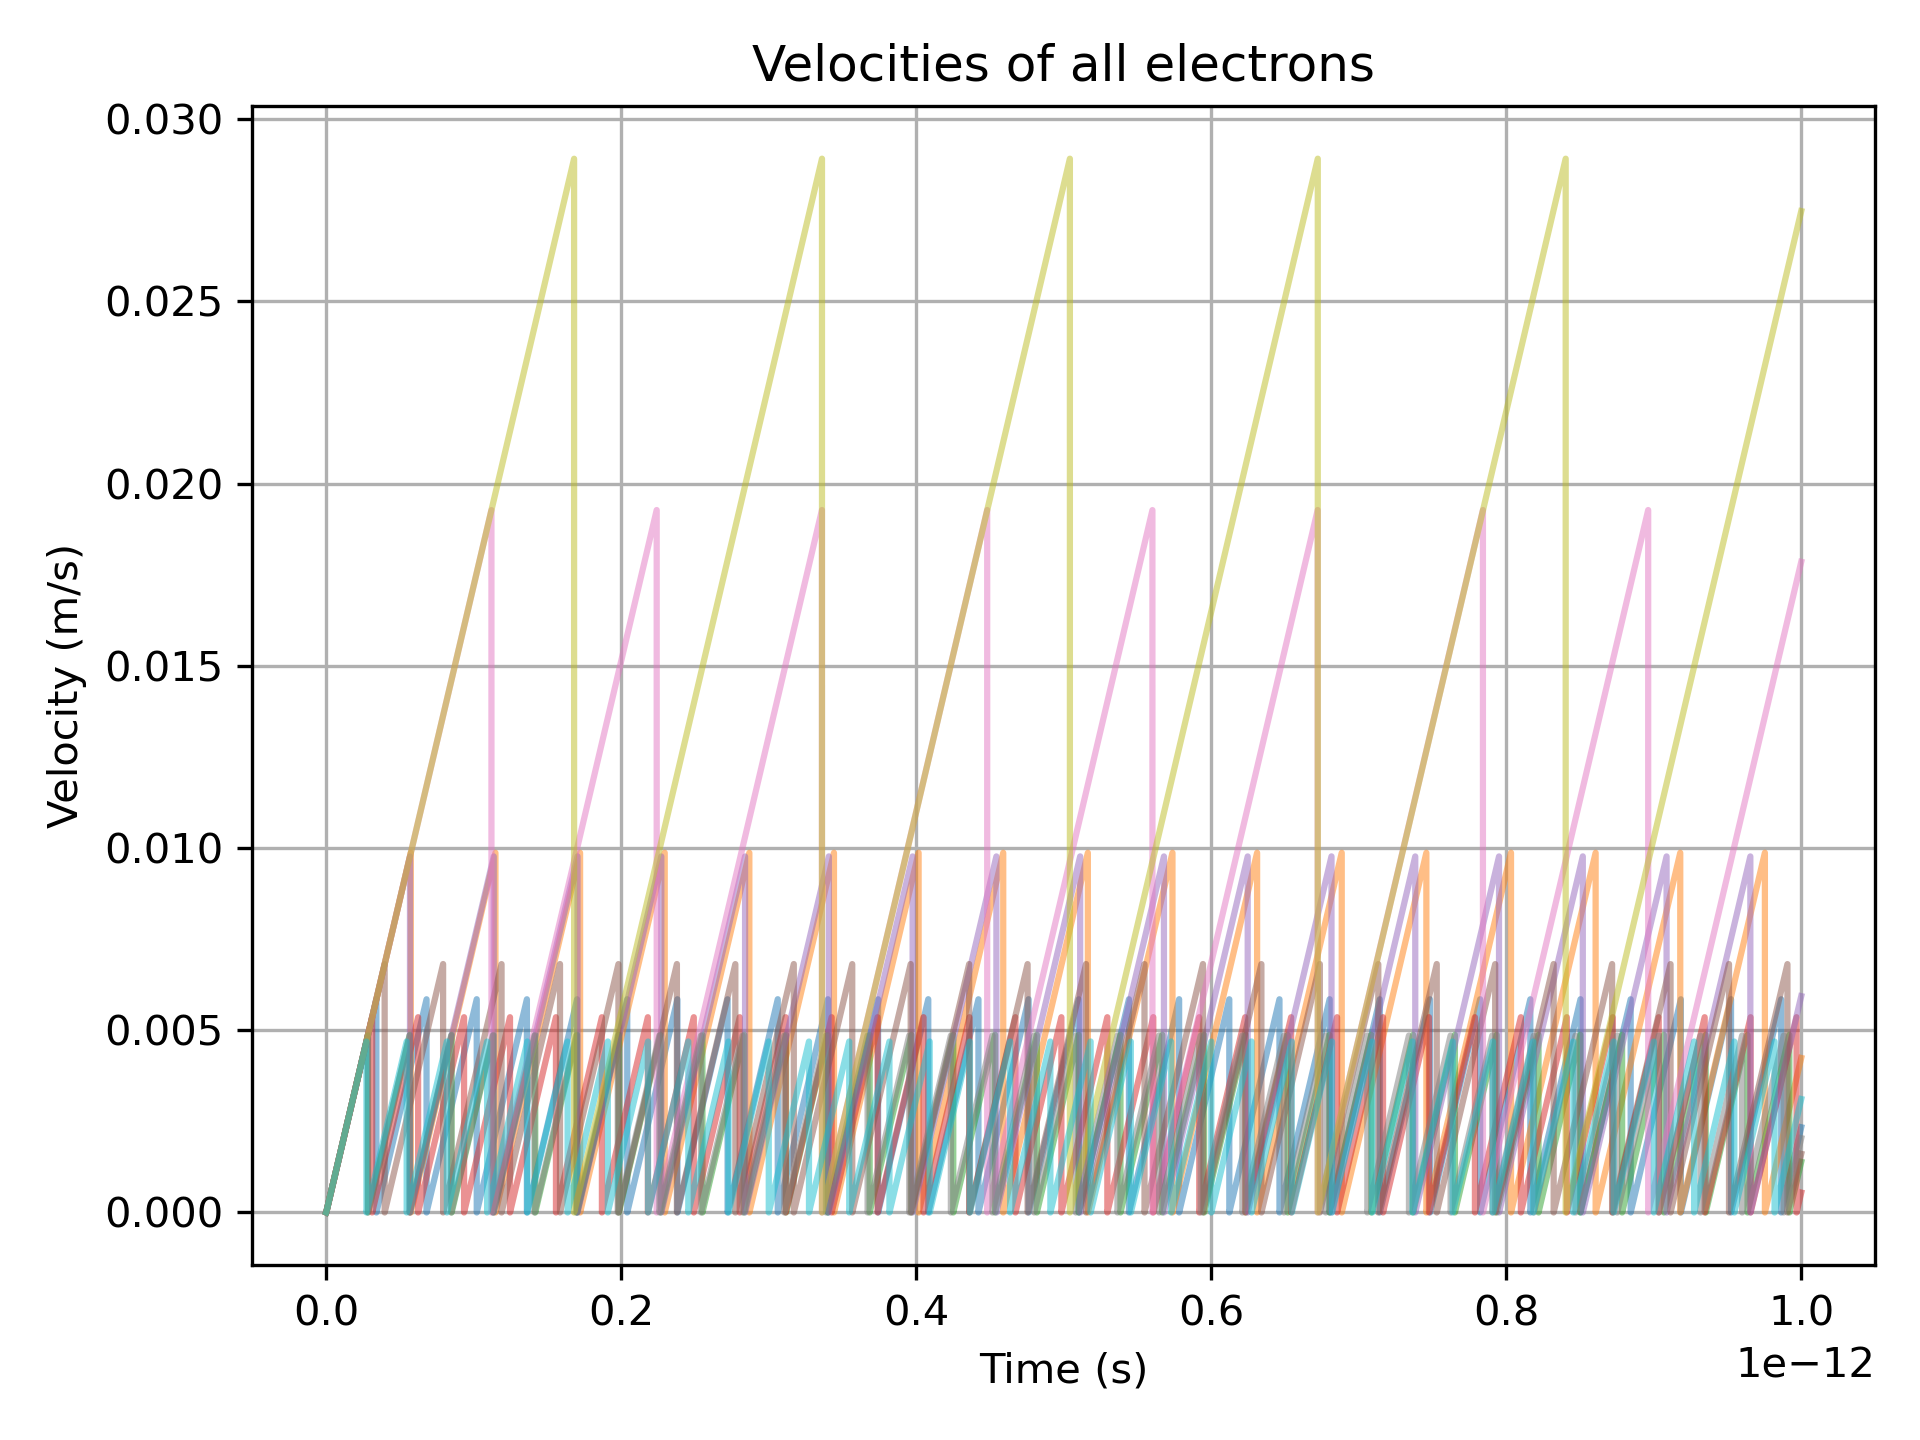
\includegraphics[width=0.48\textwidth]{figures/multi_electron_velocity.png}
\hfill
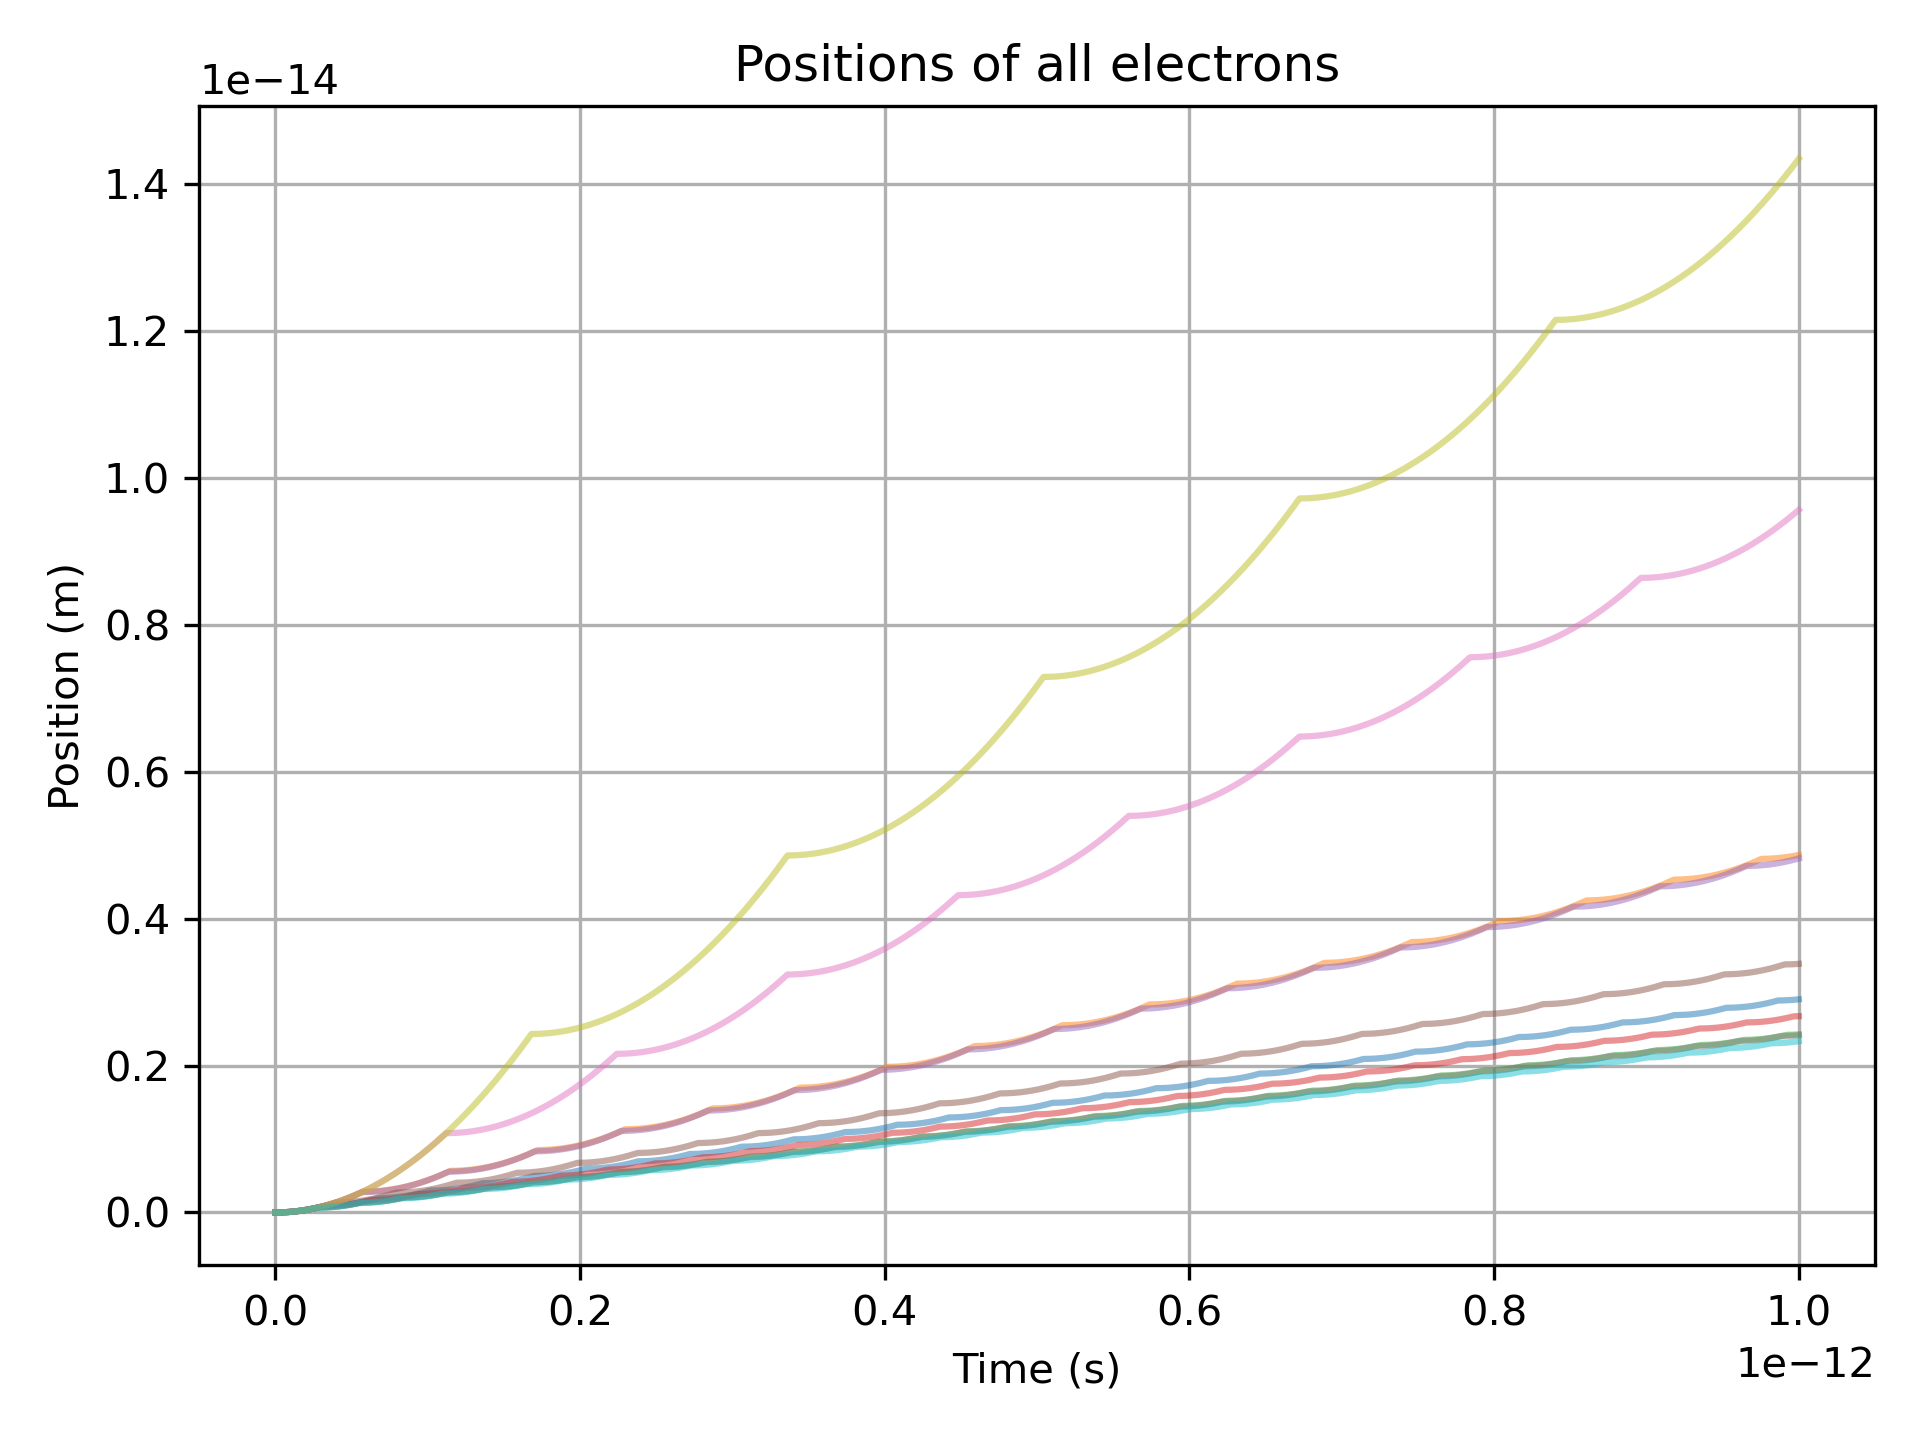
\includegraphics[width=0.48\textwidth]{figures/multi_electron_position.png}
\end{figure}
da cui si nota comunque l'andamento a "dente di sega" della velocità, e il corrispettivo comportamento dello spostamento, al variare del tempo di cammino impostato per ogni elettrone.

Un risultato molto più utile si ha tracciando la velocità media di tutti gli elettroni ad ogni istante temporale. Inoltre, il modello si comporta molto meglio prendendo un numero elevato di elettroni. Poniamo quindi $100$ elettroni e tracciamo il grafico della velocità media:
\begin{figure}[H]
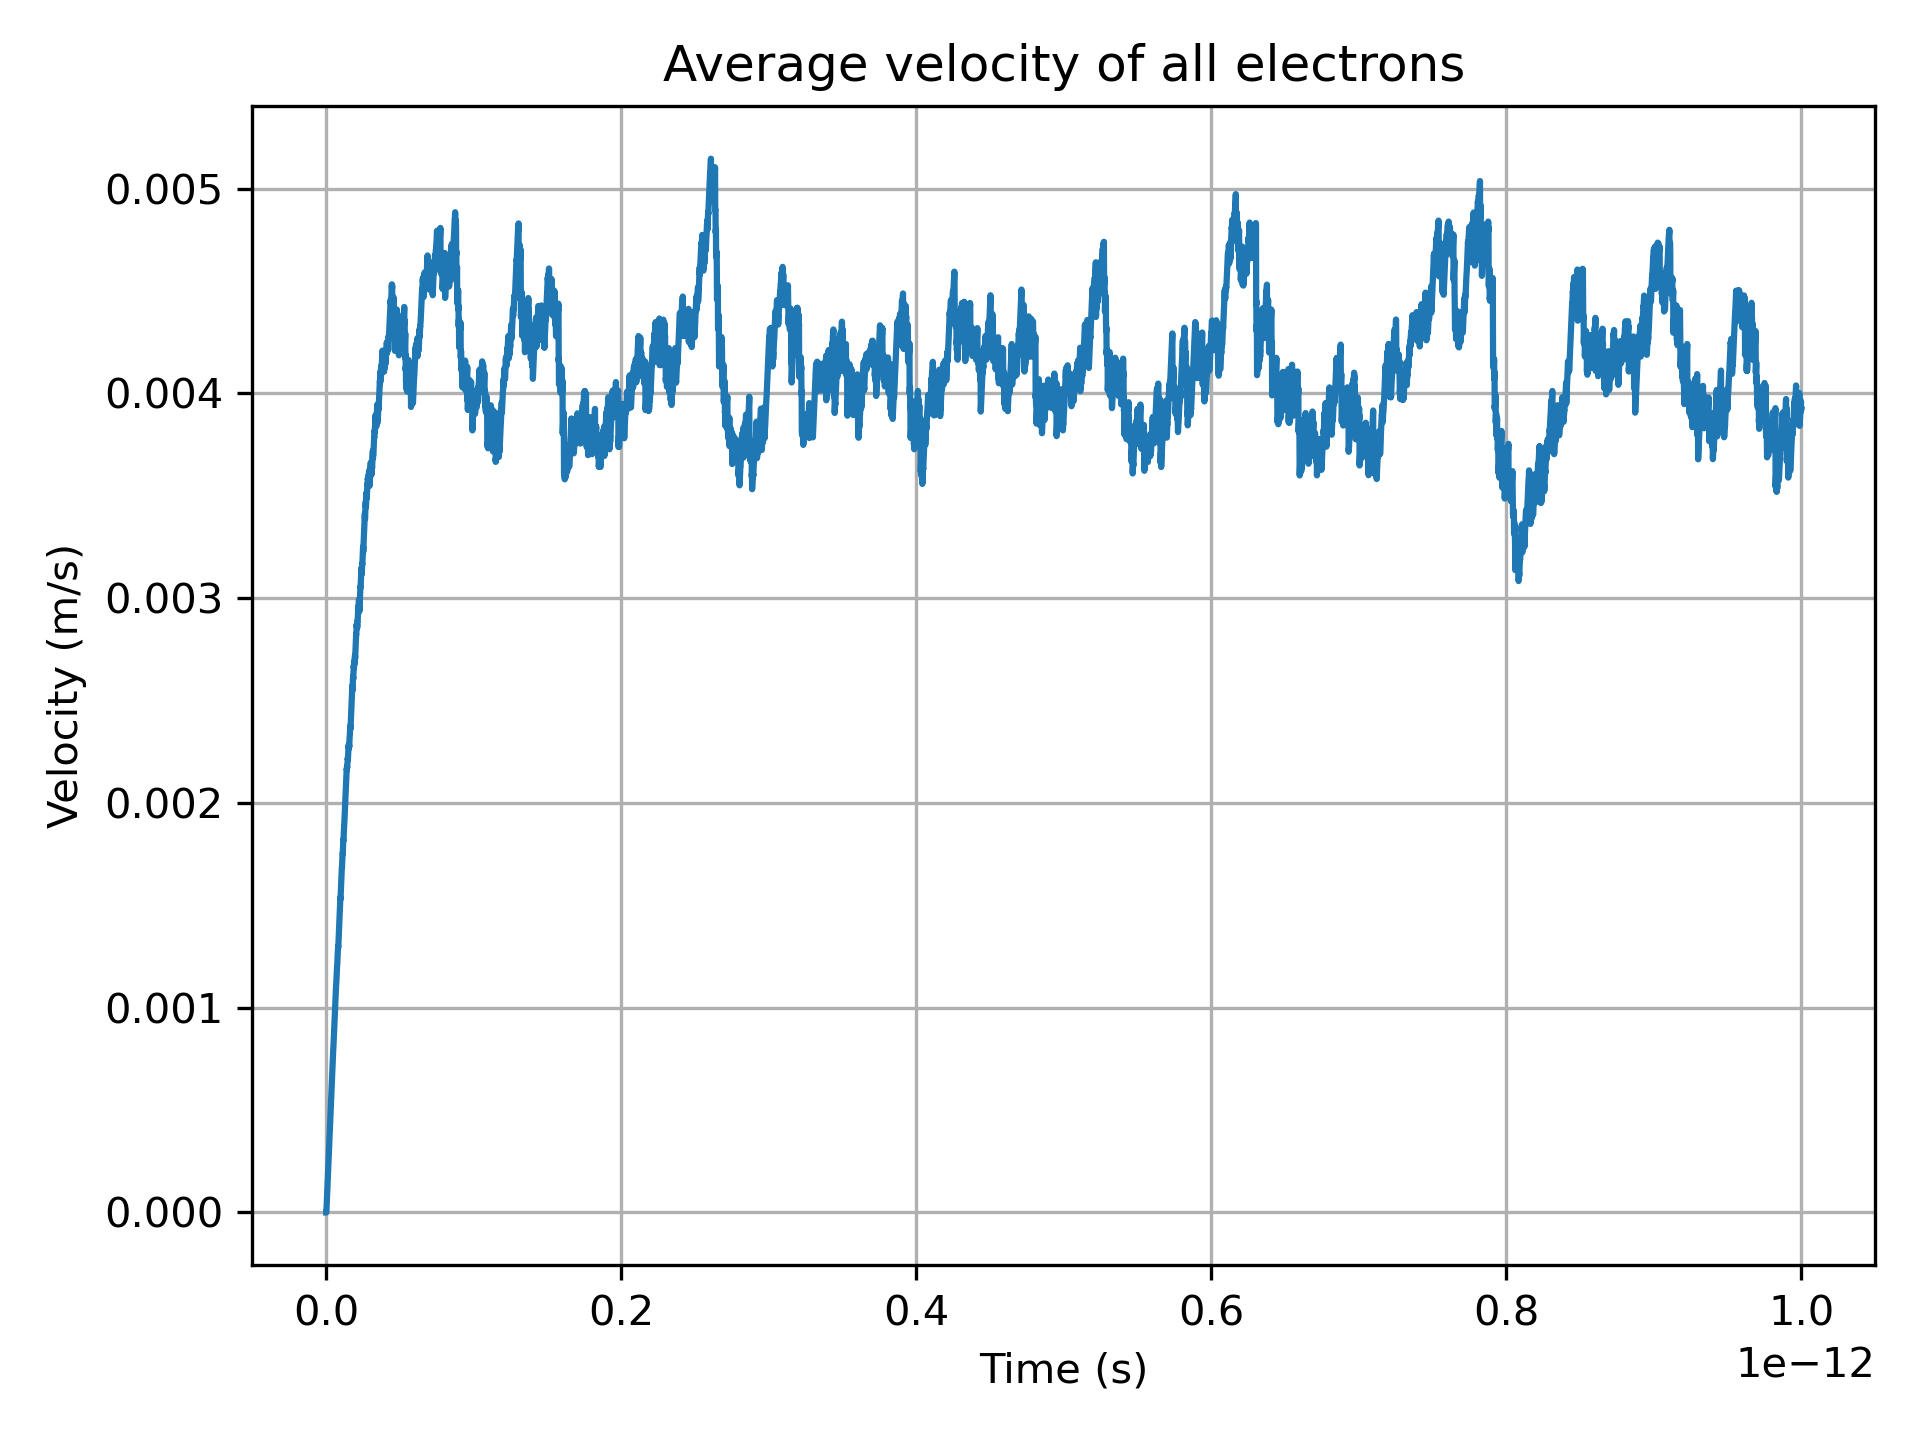
\includegraphics[width=0.96\textwidth]{figures/multi_electron_avg_velocity.png}
\end{figure}
Da questo grafico si nota che il valore medio della velocità oscilla attorno alla media che ci aspettiamo di ottenere, cioè:
$$
v_d = \frac{q E}{m} \tau = \alpha t \approx 0.0043 \, \frac{\mathrm{m}}{\mathrm{s}} 
$$

Questo è un risultato che ci soddisfa, e che possiamo ulteriormente confermare graficando la distribuzione delle velocità come istogramma: 
\begin{figure}[H]
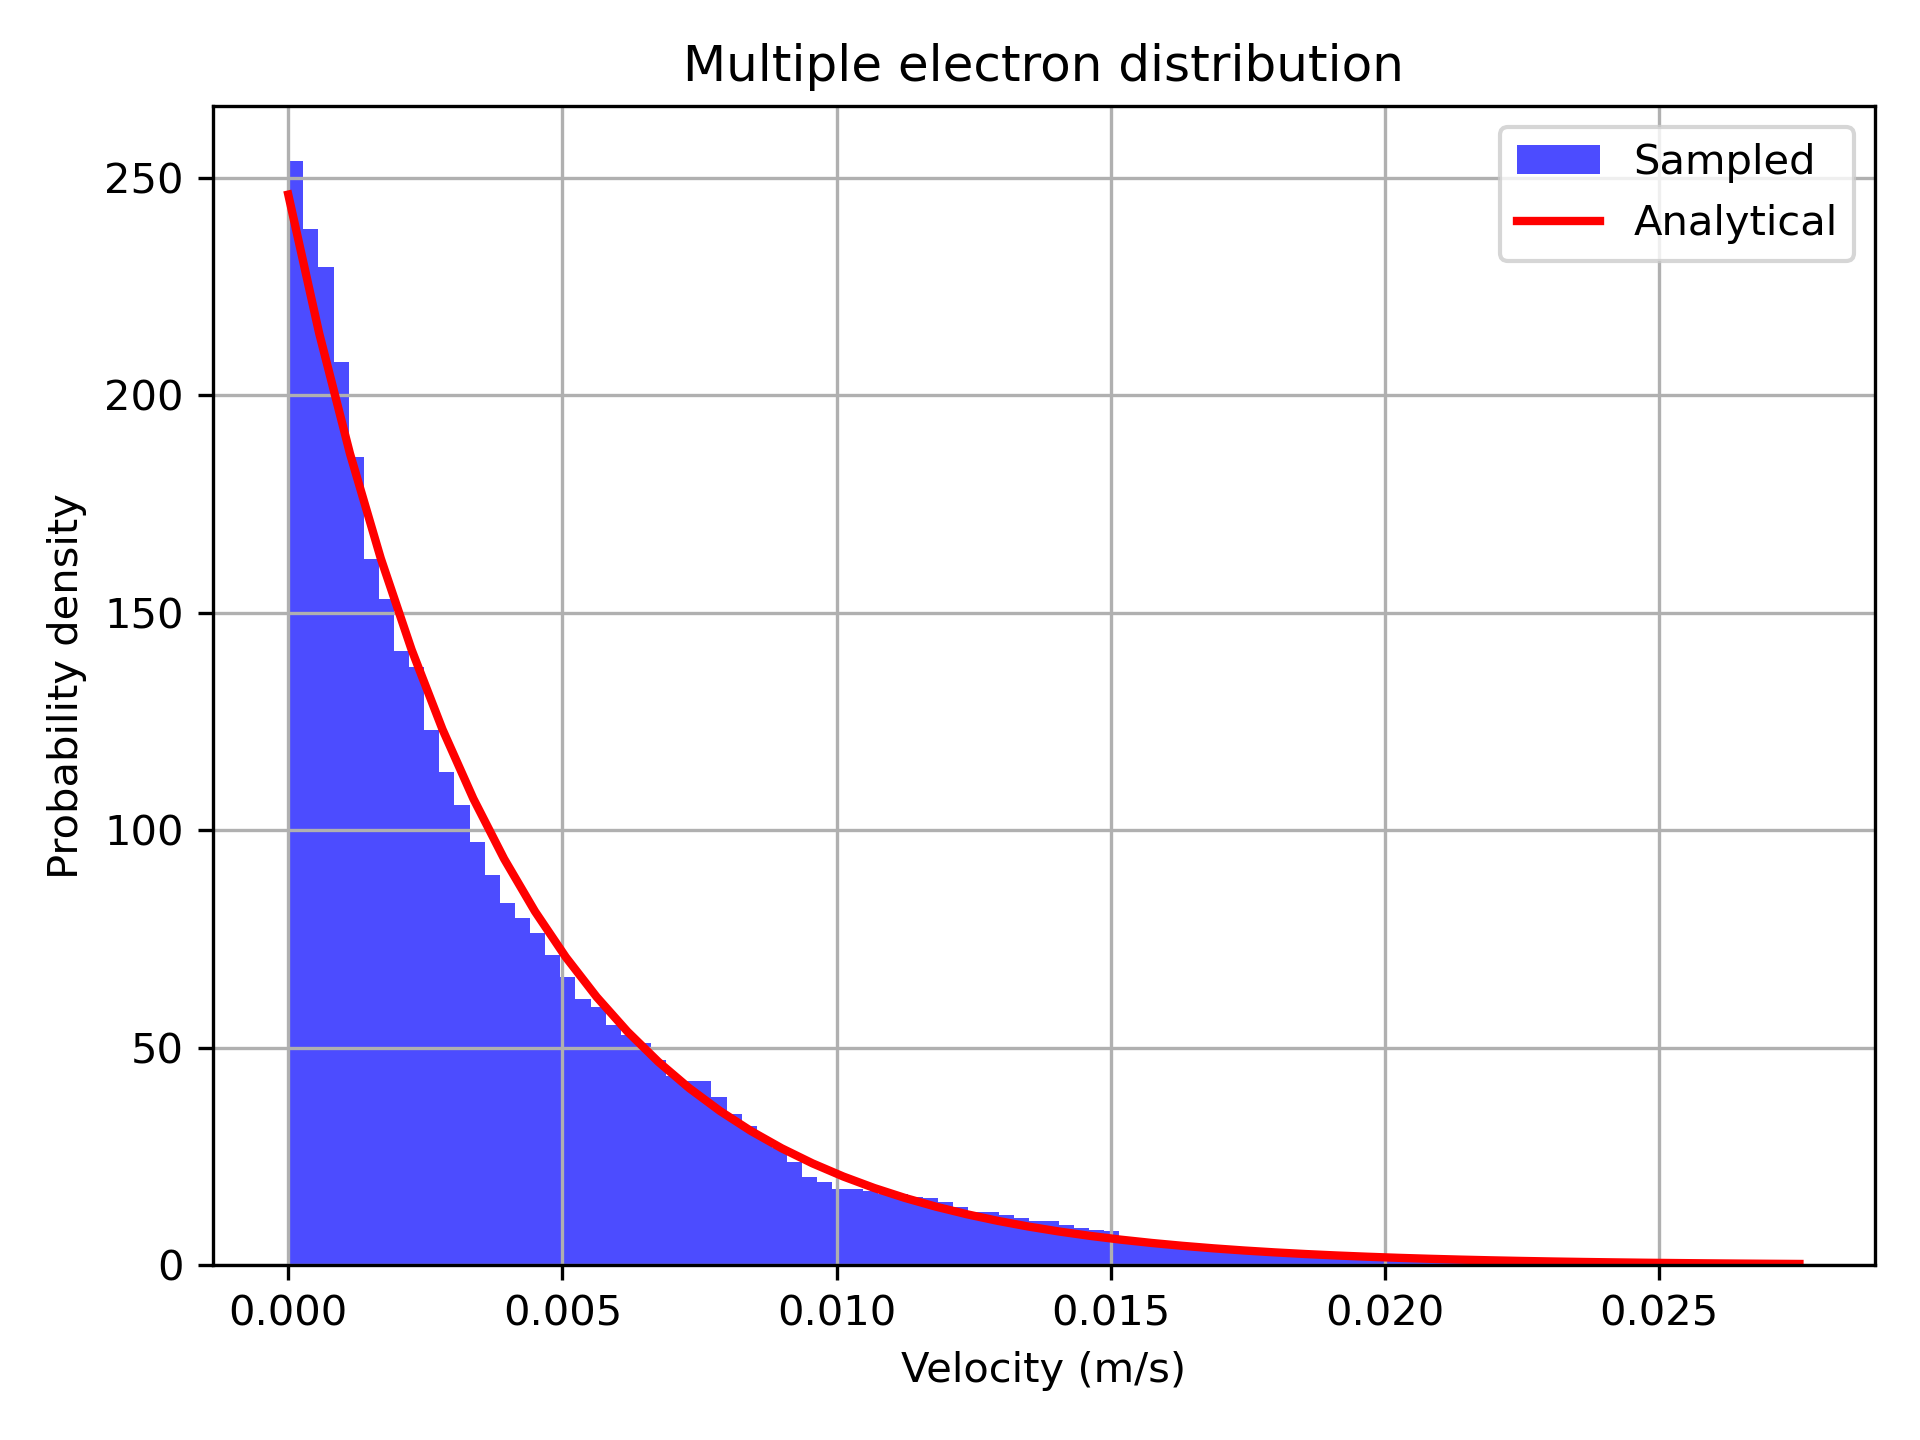
\includegraphics[width=0.96\textwidth]{figures/multi_electron_distrib.png}
\end{figure}
Anche su questo grafico è stata messa a confronto la funzione densità di probabilita della distribuzione di probabilità esponenziale con media $v_d$, cioè corrispondente alla velocità di deriva teorizzata:
$$
P(v) = \frac{1}{v_d} e^{-\frac{v}{v_d}} , \quad v_d = \frac{q E}{m} \tau = \alpha t
$$
per cui abbiamo che anche questo  modello sviluppato è in accordo con il risultato teorico, e la velocità di deriva risulta uguale all'accelerazione $a$ per il tempo di cammino medio $\tau$.

\end{document}
